\documentclass{sbc2023}

\usepackage{graphicx}
\usepackage[misc,geometry]{ifsym}
\usepackage{fontspec}
\usepackage{fontawesome}
\usepackage{academicons}
\usepackage{color}
\usepackage{hyperref}
\usepackage{aas_macros}
\usepackage[bottom]{footmisc}
\usepackage{url}
\usepackage{subcaption}
\usepackage{booktabs}
\usepackage{amsmath}
\usepackage{listings} % Adicionado para corrigir o estouro de texto do código

% Configuração do ambiente de código para não estourar a coluna
\lstset{
    basicstyle=\ttfamily\footnotesize,
    breaklines=true,
    frame=single,
    extendedchars=true,
    literate={--}{{-{}-}}2,
    columns=fullflexible
}

\setcitestyle{square}

\definecolor{orcidlogo}{rgb}{0.37,0.48,0.13}
\definecolor{unilogo}{rgb}{0.16, 0.26, 0.58}
\definecolor{maillogo}{rgb}{0.58, 0.16, 0.26}
\definecolor{darkblue}{rgb}{0.0,0.0,0.0}
\hypersetup{colorlinks,breaklinks,
            linkcolor=darkblue,urlcolor=darkblue,
            anchorcolor=darkblue,citecolor=darkblue}

\jid{}
\jtitle{Trabalho Prático - Teoria de Grafos e Computabilidade, 2026/1,}
\doi{}
\copyrightstatement{Pontifícia Universidade Católica de Minas Gerais (PUC Minas)}
\jyear{2026}

\title[Graph-Based Image Segmentation]{Análise Comparativa de Algoritmos de Segmentação de Imagens Baseados em Grafos}

\author[Equipe de Teoria de Grafos - PUC Minas]{
\affil{\textbf{Bruna Furtado}~\href{https://github.com/cestpassion}{\textcolor{black}{\faGithub}}~\textcolor{blue}{\faEnvelopeO}~~[~\textbf{Pontifícia Universidade Católica de Minas Gerais}~|\href{mailto:brunafurfon@gmail.com}{~\textbf{\textit{brunafurfon@gmail.com}}}~]}

\affil{\textbf{Domynic Barros Lima}~\href{https://github.com/DomynicBl}{\textcolor{black}{\faGithub}}~\textcolor{blue}{\faEnvelopeO}~~[~\textbf{Pontifícia Universidade Católica de Minas Gerais}~|\href{mailto:domynicbarroslima@gmail.com}{~\textbf{\textit{domynicbarroslima@gmail.com}}}~]}

\affil{\textbf{Felipe Guerzoni}~\href{https://github.com/flp2113}{\textcolor{black}{\faGithub}}~\textcolor{blue}{\faEnvelopeO}~~[~\textbf{Pontifícia Universidade Católica de Minas Gerais}~|\href{mailto:felipe.maia2113@gmail.com}{~\textbf{\textit{felipe.maia2113@gmail.com}}}~]}

\affil{\textbf{Felipe Mizher}~\href{https://github.com/FelipeMizher}{\textcolor{black}{\faGithub}}~\textcolor{blue}{\faEnvelopeO}~~[~\textbf{Pontifícia Universidade Católica de Minas Gerais}~|\href{mailto:Feliperivettimizher@gmail.com}{~\textbf{\textit{Feliperivettimizher@gmail.com}}}~]}

\affil{\textbf{Gabriel Henrique}~\href{https://github.com/GabrielDev0001}{\textcolor{black}{\faGithub}}~~[~\textbf{Pontifícia Universidade Católica de Minas Gerais}~|\href{mailto:gabrielhenriquemorais341@gmail.com}{~\textbf{\textit{gabrielhenriquemorais341@gmail.com}}}~]}

\affil{\textbf{Marcos Paulo}~\href{https://github.com/MarcosVettel}{\textcolor{black}{\faGithub}}~\textcolor{blue}{\faEnvelopeO}~~[~\textbf{Pontifícia Universidade Católica de Minas Gerais}~|\href{mailto:marcos.miranda.pereira2006@gmail.com}{~\textbf{\textit{marcos.miranda.pereira2006@gmail.com}}}~]}

\affil{\textbf{Matheus Felipe}~\href{https://github.com/mioj0kt}{\textcolor{black}{\faGithub}}~\textcolor{blue}{\faEnvelopeO}~~[~\textbf{Pontifícia Universidade Católica de Minas Gerais}~|\href{mailto:matheus.f.c.xavier2006@gmail.com}{~\textbf{\textit{matheus.f.c.xavier2006@gmail.com}}}~]}

\affil{\textbf{Paulo Gabriel}~\href{https://github.com/paulogab2601}{\textcolor{black}{\faGithub}}~\textcolor{blue}{\faEnvelopeO}~~[~\textbf{Pontifícia Universidade Católica de Minas Gerais}~|\href{mailto:Paulogabriel9002@gmail.com}{~\textbf{\textit{Paulogabriel9002@gmail.com}}}~]}

}

\begin{document}

\begin{frontmatter}
\maketitle

{\renewcommand{\faEnvelopeO}{}
\begin{mail}
Pontifícia Universidade Católica de Minas Gerais, Belo Horizonte, MG, Brasil.
\end{mail}}

\begin{dates}
\small{\textbf{Disciplina:} Teoria de Grafos e Computabilidade~~~$\bullet$~~~\textbf{Período:} 2026/1}
\end{dates}

\begin{abstract}
\textbf{Abstract.~}
This work implements and compares three graph-based image segmentation algorithms: Felzenszwalb & Huttenlocher (F&H), Cousty \emph{et al.}, and the \emph{Image Foresting Transform} (IFT). All three model the image as a weighted graph and partition its vertices, differing in their optimization strategy and degree of automation. F&H produces automatic partitions via an adaptive predicate over the MST; Cousty offers hierarchical control through cuts at different thresholds on the same MST, exporting a saliency map; IFT propagates conquest boundaries from seeds, being precise when these are strategically positioned. Experiments with five color and grayscale images show complementary profiles: F&H is effective in simple scenes, Cousty is the most versatile, and IFT excels in interactive object extraction. The code was implemented in C++17 and is available in the project's repository.
\end{abstract}

\begin{keywords}
Segmentação de Imagens, Grafos, Árvore Geradora Mínima, Image Foresting Transform, Quasi-Flat Zones
\end{keywords}

\end{frontmatter}

% ─────────────────────────────────────────────────────────────────────────────
\section{Introdução}
\label{sec:intro}
\vspace*{-8pt}
A segmentação de imagens consiste em particionar uma imagem digital em regiões
cujos pixels compartilham características visuais — cor, intensidade ou textura
— de modo que regiões adjacentes apresentem diferenças significativas. Aplicações
abrangem diagnóstico médico, navegação autônoma e edição de conteúdo digital.
A modelagem via teoria de grafos transforma o problema em particionamento de
vértices: cada pixel é um vértice $v \in V$, pares de vizinhos são ligados por
arestas ponderadas pela dissimilaridade $w(v_i, v_j)$, e os componentes conexos
resultantes correspondem aos segmentos finais \citep{felzenszwalb2004}.
Este trabalho implementa e compara três métodos canônicos:
\textbf{(a)}~F\&H, baseado em Árvore Geradora Mínima (MST) com predicado
adaptativo \citep{felzenszwalb2004};
\textbf{(b)}~Cousty \emph{et al.}, segmentação hierárquica via quasi-flat zones
sobre a MST \citep{cousty2018}; e
\textbf{(c)}~IFT, baseada em caminho mínimo com múltiplas sementes
\citep{falcao2004}.
A implementação em C++17 usa vizinhança de 8~conexões e a biblioteca
\texttt{stb\_image} para entrada/saída. O peso de cada aresta é a distância
Euclidiana no espaço RGB (imagens coloridas) ou a diferença absoluta de
intensidade (escala de cinza).

% ─────────────────────────────────────────────────────────────────────────────
\section{Fundamentação e Metodologia}
\label{sec:metodo}

\subsection{Felzenszwalb \& Huttenlocher (F\&H)}

O algoritmo F\&H \citep{felzenszwalb2004} adota abordagem aglomerativa
(\emph{bottom-up}) derivada do algoritmo de Kruskal. As arestas são ordenadas
em peso crescente, para cada aresta conectando dois componentes $C_1$ e $C_2$,
avalia-se o predicado de fusão:
\[
  \mathrm{Dif}(C_1, C_2) \leq \mathrm{MInt}(C_1, C_2),
\]
onde $\mathrm{Dif}(C_1, C_2)$ é o peso da aresta de menor custo conectando os dois componentes e o limite interno $\mathrm{MInt}$ é definido como:
\begin{equation}
    \mathrm{MInt}(C_1, C_2) = \min(\mathrm{Int}(C_1) + \tau(C_1), \mathrm{Int}(C_2) + \tau(C_2)).
\end{equation}

Aqui, $\mathrm{Int}(C)$ é o maior peso da MST interna ao componente e $\tau(C)=k/|C| $ é um limiar adaptativo que inibe a criação de segmentos pequenos. O parâmetro $k$ controla a granularidade global. A estrutura \emph{Disjoint-Set Union} (DSU) com compressão de caminho garante desempenho quase linear em $O(m \log m)$, onde $m$ é o número de arestas.

\subsection{Cousty \emph{et al.} — Segmentação Hierárquica por Quasi-Flat Zones}

O método de Cousty \citep{cousty2018} constrói uma única MST via Kruskal e
realiza cortes hierárquicos sobre ela. Dado um limiar $t$, mantêm-se apenas as
arestas com $w \leq t$; a floresta resultante define os componentes. Esse
procedimento implementa o conceito de \emph{quasi-flat zones}: regiões onde
nenhum caminho interno excede o limiar $t$. A MST é construída uma única vez,
e diferentes valores de $t$ produzem toda a hierarquia de segmentações sem
reprocessar o grafo original — vantagem computacional expressiva em relação a
executar F\&H múltiplas vezes com parâmetros distintos.

O \textbf{mapa de saliência} é gerado normalizando para $[0,255]$ o maior peso
incidente em cada vértice da MST. Regiões homogêneas aparecem escuras e
fronteiras de objetos formam contornos claros (Figura~\ref{fig:resultados},
linha~3), revelando a estrutura hierárquica da imagem sem qualquer limiar
definido a priori.

\subsection{Image Foresting Transform (IFT)}

A IFT \citep{falcao2004} reformula a segmentação como competição entre sementes
(\emph{seeds}) para conquistar pixels por caminhos de custo mínimo, análoga ao
algoritmo de Dijkstra para múltiplas fontes. A função de custo $f_{\max}$ define:
\[
  f_{\max}(\pi \cdot \langle s,t \rangle) = \max\{f_{\max}(\pi),\; w(s,t)\}.
\]
Sementes recebem custo zero; demais pixels recebem custo infinito. Uma fila de
prioridades (\emph{min-heap}) processa iterativamente o pixel de menor custo,
atualizando vizinhos. O segmento de cada pixel é determinado pela semente que o
alcança pelo caminho de menor custo máximo. O \textbf{mapa de custos} exportado
visualiza esses valores, revelando quais regiões são barreiras para a propagação.

\subsection{Pipeline Experimental}

Os três algoritmos operam sobre a mesma representação de grafo. Um filtro de
mediana $3{\times}3$ é aplicado opcionalmente antes da segmentação para atenuar
ruído impulsivo sem degradar bordas — especialmente relevante para F\&H e Cousty,
cujos critérios são sensíveis a variações locais de intensidade. Para cada saída,
três visualizações são geradas: \texttt{\_random} (cor aleatória por segmento),
\texttt{\_avg} (cor média real da região) e \texttt{\_boundary} (bordas em
vermelho sobrepostas à imagem original). Cousty exporta adicionalmente o mapa de
saliência; a IFT, o mapa de custos.

O sistema foi implementado como um executável de linha de comando (\texttt{segmentador})
com interface unificada para os três métodos. O modo \emph{batch}
(\texttt{--batch}) processa automaticamente todas as imagens de um diretório,
gerando todas as visualizações para cada arquivo sem intervenção manual. A
Figura~\ref{fig:uso_code} ilustra os comandos utilizados nos experimentos relatados
neste trabalho.

\begin{figure}[h]
\centering
\begin{lstlisting}[language=bash]
# Felzenszwalb com filtro de mediana
./segmentador --input data/input/ --output data/output/ --method felzenszwalb --k 300 --median --batch

# Cousty com tres limiares simultaneos
./segmentador --input data/input/ --output data/output/ --method cousty --thresholds 20,40,80 --median --batch

# IFT com grade 3x3 de sementes automaticas
./segmentador --input data/input/ --output data/output/ --method ift --auto-seeds 3 3 --median --batch
\end{lstlisting}
\caption{Comandos utilizados nos experimentos em modo \emph{batch}.
  O parâmetro \texttt{--thresholds} permite gerar múltiplos níveis hierárquicos
  do Cousty em uma execução; \texttt{--auto-seeds} define uma grade
  uniforme de sementes para a IFT.}
\label{fig:uso_code}
\end{figure}

% ─────────────────────────────────────────────────────────────────────────────
\section{Resultados e Análise}
\label{sec:resultados}

Os experimentos foram conduzidos sobre cinco imagens (\texttt{alien},
\texttt{cenario}, \texttt{dados}, \texttt{flor}, \texttt{shrek}), cobrindo fundo
homogêneo, paisagem natural, objetos coloridos, cena botânica e personagem
texturizado. A Figura~\ref{fig:resultados} apresenta resultados representativos.

\paragraph{F\&H.} Em imagens com fundo homogêneo e objetos de cores sólidas
(\texttt{alien}, \texttt{dados}), o predicado adaptativo delineou corretamente as
fronteiras principais. Em cenas ricas em textura ou gradiente suave
(\texttt{cenario}, \texttt{flor}, \texttt{shrek}), ocorreu super-segmentação
severa: pequenas variações locais excedem rapidamente o $\mathrm{Int}(C)$ dos
componentes emergentes, inibindo fusões e gerando centenas de segmentos espúrios.
O filtro de mediana reduziu consideravelmente esse efeito.

\paragraph{Cousty.} Testado com $t \in \{20, 40, 80\}$, demonstrou controle
hierárquico preciso. Com $t{=}20$, bordas sutis são preservadas (resultado
similar ao F\&H, porém mais limpo). Com $t{=}80$, regiões homogêneas coalescem
em grandes blocos semânticos: para \texttt{cenario}, isolou corretamente céu,
árvore, vegetação e caminho; para \texttt{alien}, separou o personagem do fundo
com dois segmentos dominantes; para \texttt{flor}, agrupou pétalas por faixa de
cor ignorando as listras internas. O mapa de saliência revelou, de forma
consistente entre todas as imagens, que os pesos mais altos da MST coincidem com
as fronteiras perceptualmente relevantes.

\paragraph{IFT.} Com sementes posicionadas automaticamente nos cantos da imagem,
o IFT produziu segmentações triviais na maioria dos casos: a semente no canto de
uma região homogênea grande (fundo branco do \texttt{alien}, céu do
\texttt{cenario}) conquistou a imagem inteira antes que outras sementes pudessem
competir efetivamente. O mapa de custos confirmou esse fenômeno — pixels do
objeto apresentaram custos altos, indicando que a fronteira de alto peso da
silhueta bloqueou a propagação. A exceção foi \texttt{flor}: o fundo escuro
homogêneo fez a semente de canto convergir rapidamente para o background, e a
borda da flor atuou como barreira natural, gerando uma separação flor/fundo
precisa. Esse comportamento evidencia que a IFT foi projetada para extração interativa precisa.

\subsection{Análise do Comportamento em Escala de Cinza vs. Colorido}

O pipeline foi avaliado comparando as execuções em modo colorido (RGB) e escala de cinza (\texttt{--gray}). Essa alteração modifica diretamente a natureza matemática do cálculo do peso das arestas do grafo. Enquanto no modo colorido o peso representa a distância Euclidiana tridimensional ($\sqrt{\Delta R^2 + \Delta G^2 + \Delta B^2}$), no modo escala de cinza o espaço de características é colapsado para uma única dimensão de intensidade, calculada via diferença absoluta ($|I_1 - I_2|$).

Os experimentos revelaram que a conversão para escala de cinza atua como um filtro de atenuação de ruído cromático. Em texturas de alta frequência com matizes variados mas luminância estável (como o colete texturizado em \texttt{shrek} e as folhas de fundo em \texttt{flor}), os algoritmos de F\&H e Cousty apresentaram partições marcadamente mais estáveis e menos fragmentadas no modo cinza. O colapso de canais eliminou falsas bordas geradas por transições puramente cromáticas, permitindo que os predicados aglomerativos fizessem fusões de componentes de forma mais abrangente. Por outro lado, em cenários onde a separação semântica depende estritamente do matiz (como nos \texttt{dados} coloridos sobre fundo neutro), a escala de cinza gerou ambiguidades de peso nas fronteiras devido ao metamorfismo de luminância entre objetos distintos, degradando a precisão dos contornos obtidos pela IFT.

\begin{figure}[t]
  \centering
  \begin{subfigure}[t]{0.32\columnwidth}
    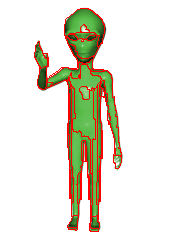
\includegraphics[width=\linewidth]{figs/alien_felzenszwalb_boundary.png}
    \caption*{\scriptsize F\&H (\texttt{alien})}
  \end{subfigure}\hfill
  \begin{subfigure}[t]{0.32\columnwidth}
    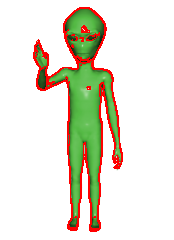
\includegraphics[width=\linewidth]{figs/alien_cousty_t20_boundary.png}
    \caption*{\scriptsize Cousty $t{=}20$}
  \end{subfigure}\hfill
  \begin{subfigure}[t]{0.32\columnwidth}
    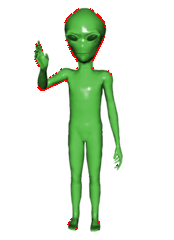
\includegraphics[width=\linewidth]{figs/alien_cousty_t80_boundary.png}
    \caption*{\scriptsize Cousty $t{=}80$}
  \end{subfigure}

  \vspace{3pt}

  \begin{subfigure}[t]{0.32\columnwidth}
    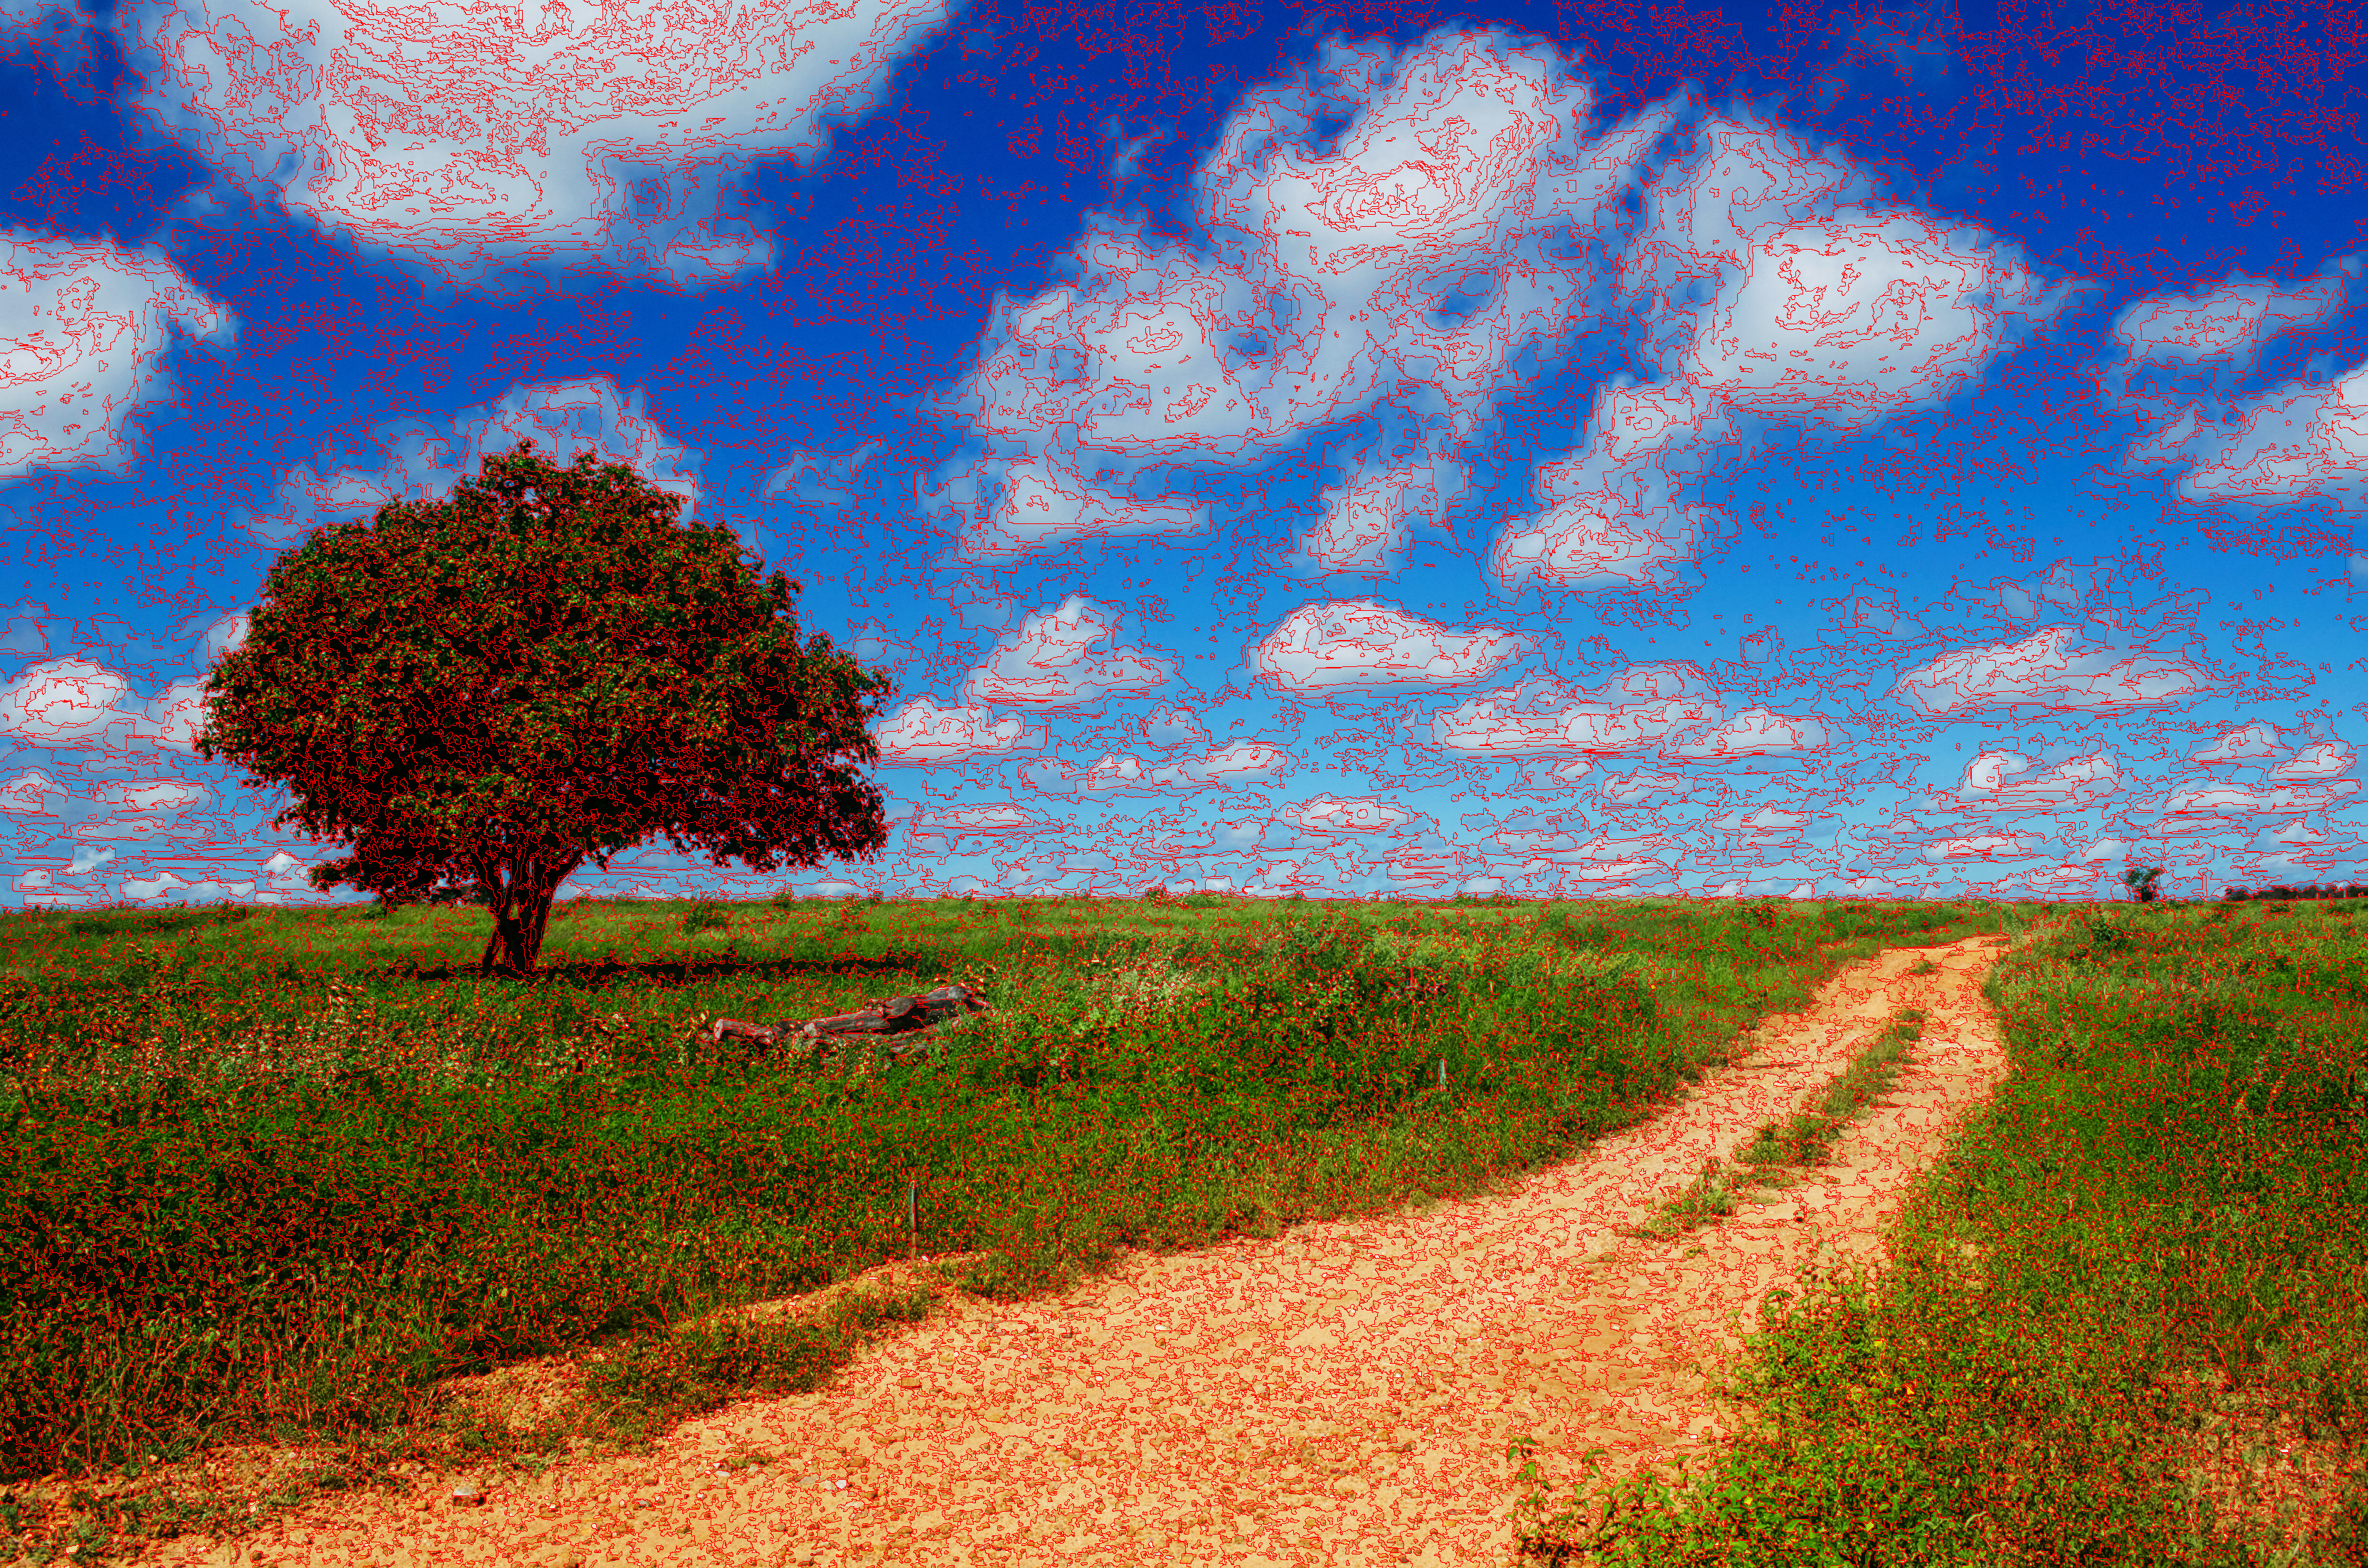
\includegraphics[width=\linewidth]{figs/cenario_felzenszwalb_boundary.png}
    \caption*{\scriptsize F\&H (\texttt{cenario})}
  \end{subfigure}\hfill
  \begin{subfigure}[t]{0.32\columnwidth}
    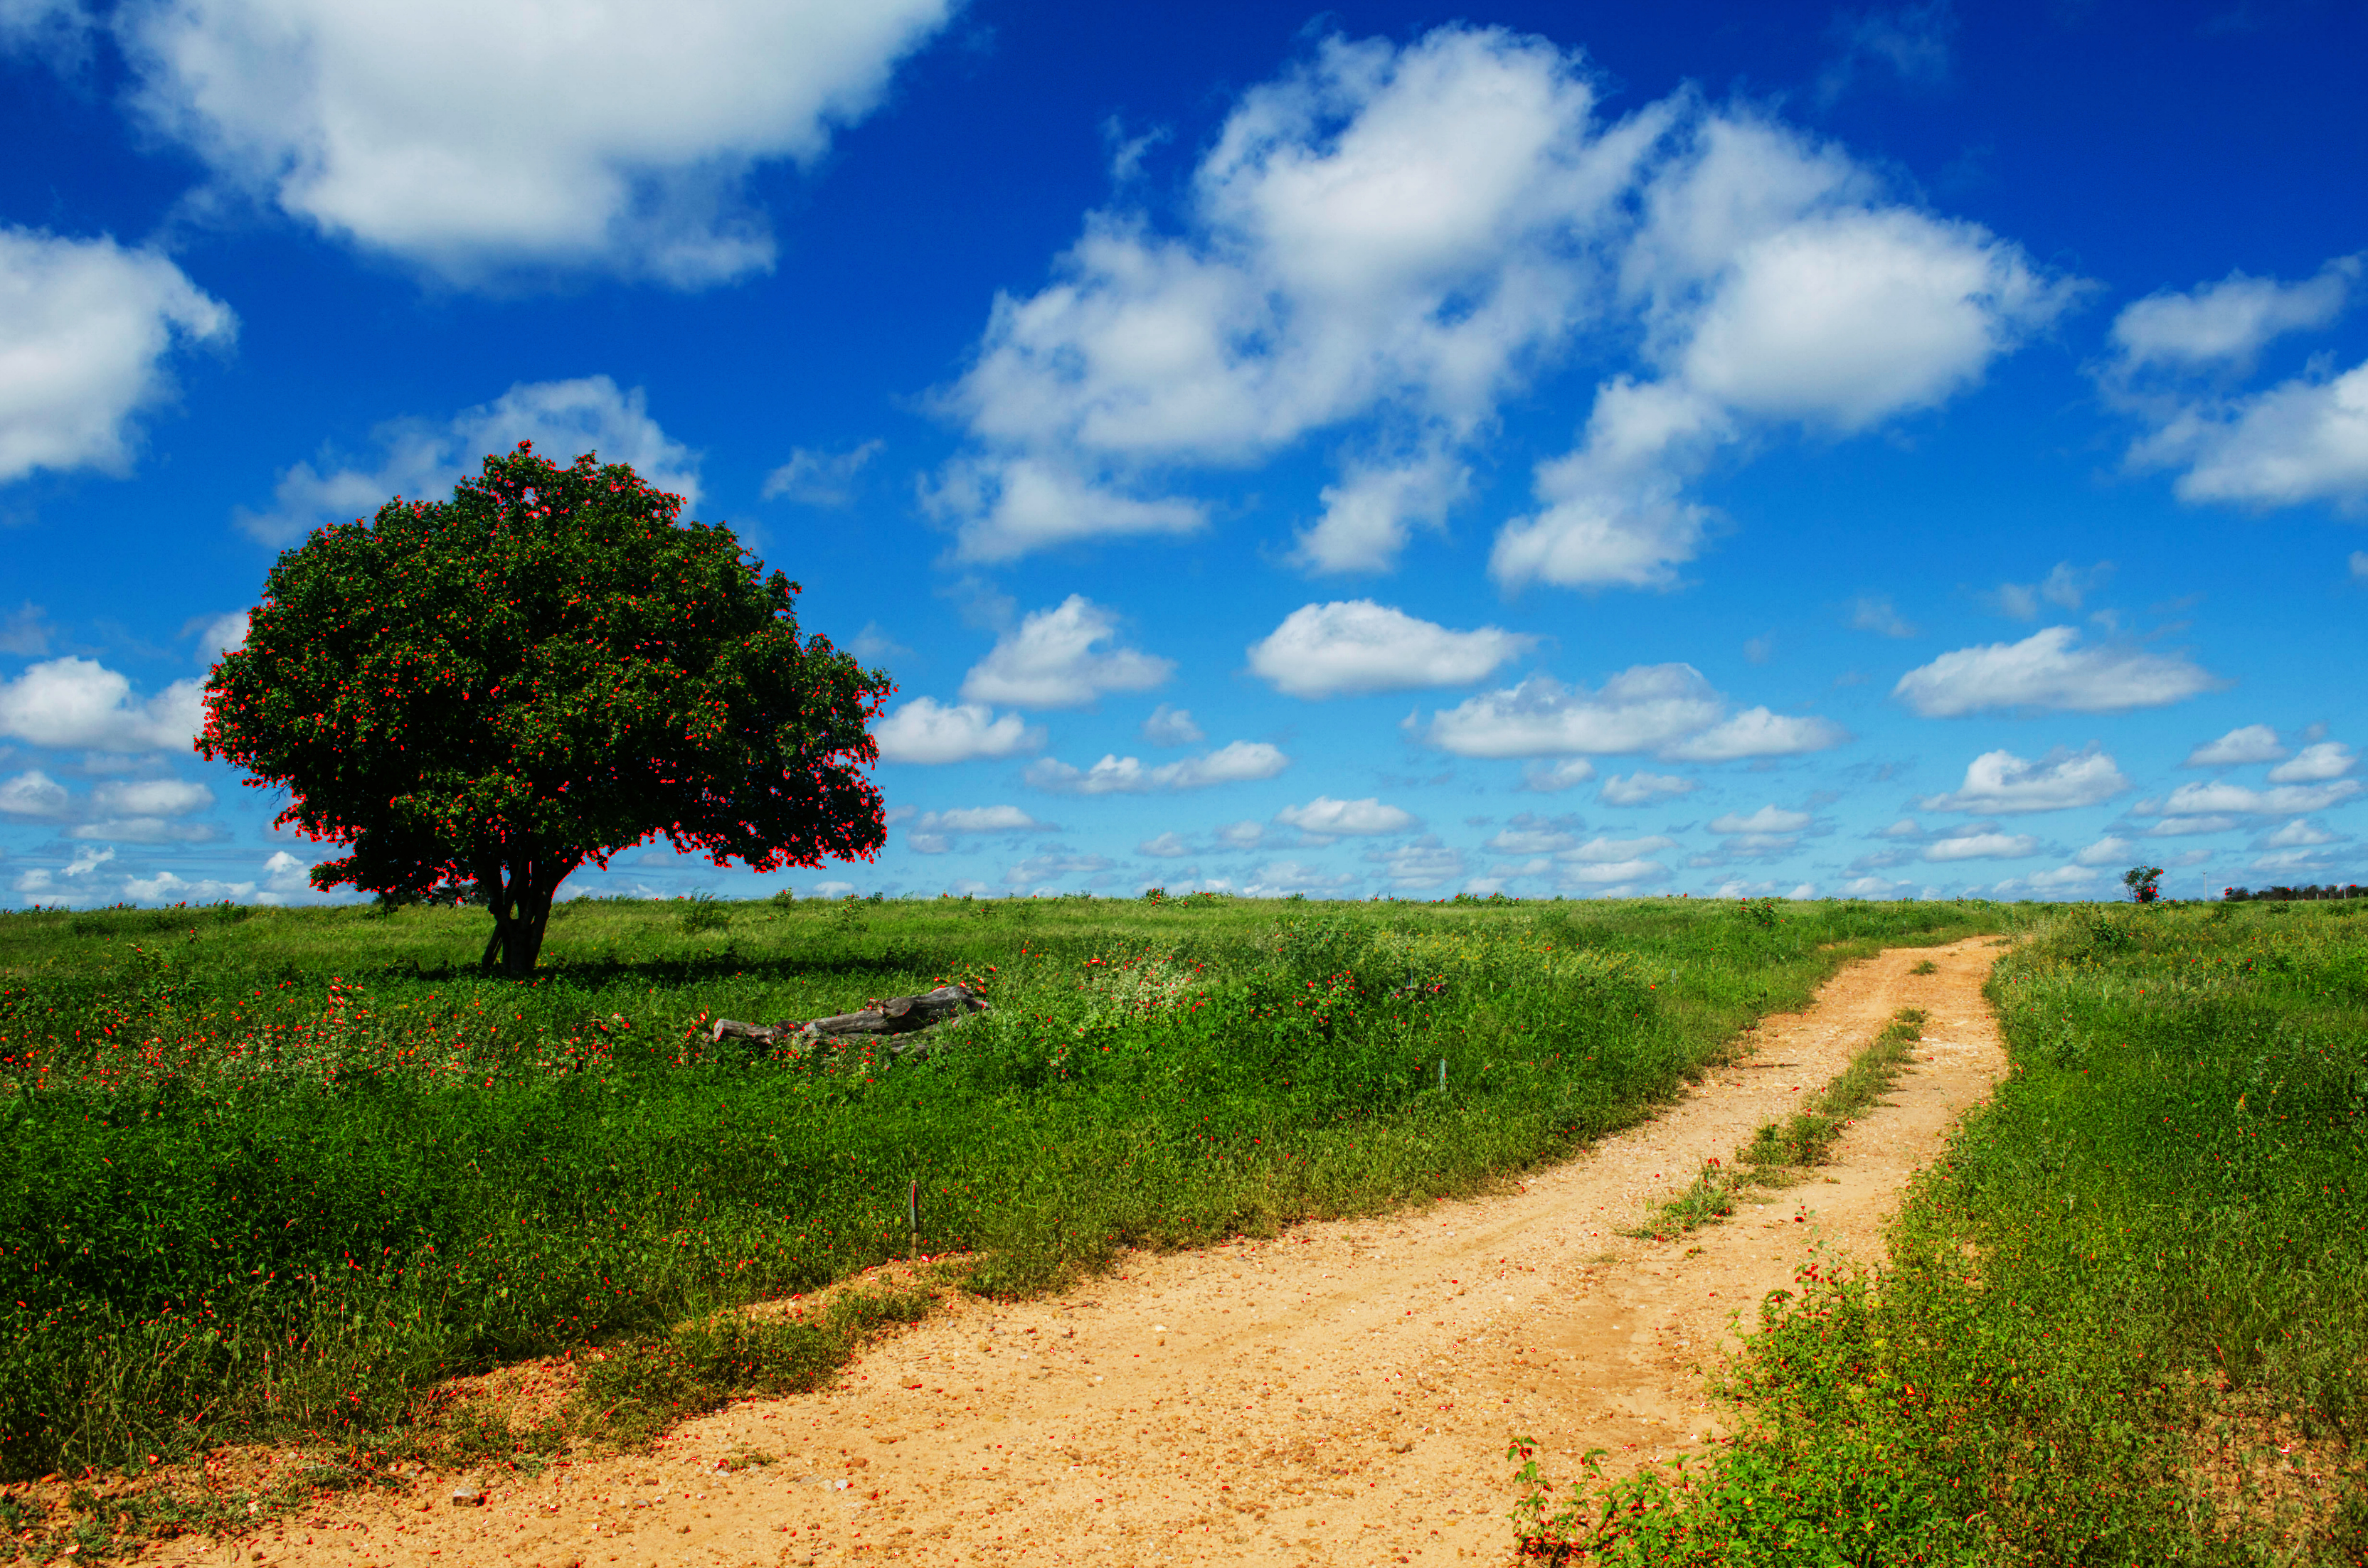
\includegraphics[width=\linewidth]{figs/cenario_cousty_t40_boundary.png}
    \caption*{\scriptsize Cousty $t{=}40$}
  \end{subfigure}\hfill
  \begin{subfigure}[t]{0.32\columnwidth}
    
\includegraphics[width=\linewidth]{figs/cenario_cousty_t80_avg.png}
    \caption*{\scriptsize Cousty $t{=}80$}
  \end{subfigure}

  \vspace{3pt}

  \begin{subfigure}[t]{0.32\columnwidth}
    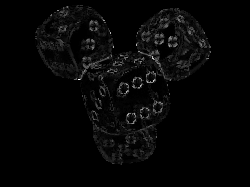
\includegraphics[width=\linewidth]{figs/dados_cousty_saliency.png}
    \caption*{\scriptsize Saliência (\texttt{dados})}
  \end{subfigure}\hfill
  \begin{subfigure}[t]{0.32\columnwidth}
    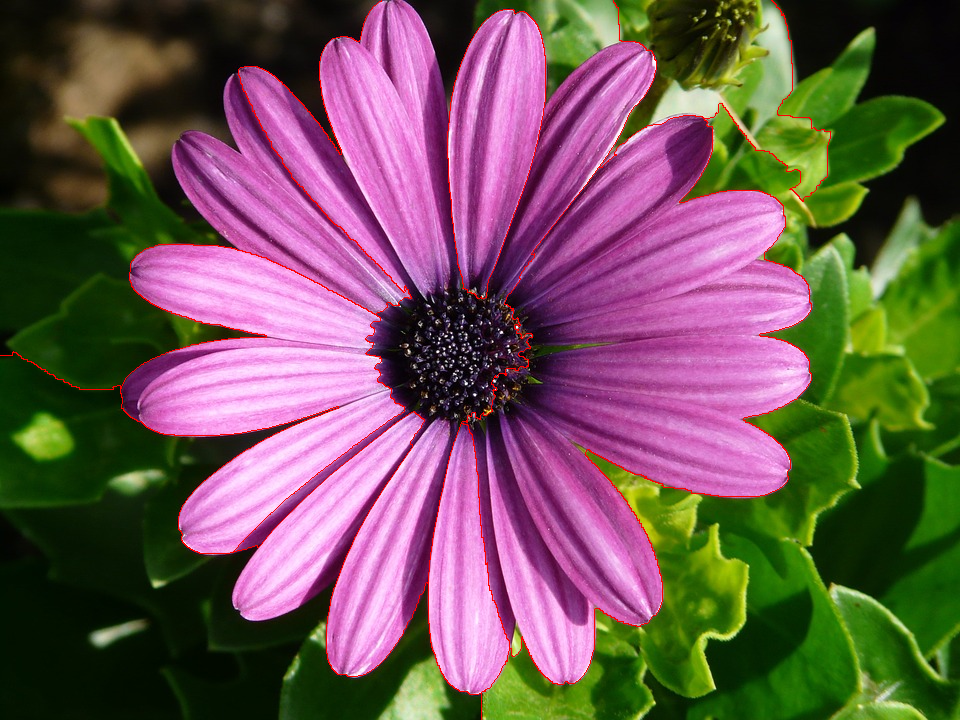
\includegraphics[width=\linewidth]{figs/flor_ift_boundary.png}
    \caption*{\scriptsize IFT (\texttt{flor})}
  \end{subfigure}\hfill
  \begin{subfigure}[t]{0.32\columnwidth}
    
\includegraphics[width=\linewidth]{figs/flor_cousty_t80_avg.png}
    \caption*{\scriptsize Cousty $t{=}80$ (\texttt{flor})}
  \end{subfigure}

  \caption{Linha~1: super-segmentação de F\&H vs.\ controle hierárquico do
    Cousty em \texttt{alien}. Linha~2: F\&H gera mosaico espúrio em cena
    natural; Cousty $t{=}80$ isola céu, vegetação e caminho com 4--5 segmentos
    semânticos. Linha~3: mapa de saliência dos \texttt{dados} com bordas claras
    nos contornos reais; melhor caso da IFT (\texttt{flor}, fundo escuro
    homogêneo) e resultado hierárquico do Cousty na mesma imagem.}
  \label{fig:resultados}
\end{figure}

\subsection{Comparativo e Correlação entre os Métodos}

Os três métodos compartilham a abstração de grafo ponderado, mas diferem
fundamentalmente na estratégia de otimização (Tabela~\ref{tab:comp}). F\&H e
Cousty são correlatos: ambos processam as arestas da MST em ordem crescente de
peso e usam DSU para manter componentes. A diferença essencial é que F\&H aplica
um predicado \emph{local e adaptativo} que evolui com o tamanho dos componentes,
enquanto Cousty realiza um \emph{corte global} a um limiar fixo sobre a MST
pré-construída — gerando toda a hierarquia de segmentações sem reprocessar o
grafo. A IFT difere fundamentalmente: em vez de agregar componentes, ela propaga
fronteiras de conquista a partir de fontes externas, otimizando o custo de
caminho máximo de cada pixel a sua semente mais próxima. A correlação entre os
métodos está na representação compartilhada: todos traduzem o problema visual
de segmentação para o domínio matemático da teoria dos grafos, e o mapa de
saliência do Cousty e o mapa de custos da IFT revelam, de formas distintas, a
mesma estrutura subjacente de pesos da MST.

\begin{table}[t]
\caption{Comparativo das metodologias de segmentação.}
\label{tab:comp}
\centering
\small
\begin{tabular}{@{}lccc@{}}
\hline\hline
 & \textbf{F\&H} & \textbf{Cousty} & \textbf{IFT} \\
\hline
Base          & MST           & MST + corte     & Caminho mín.  \\
Lógica        & Aglomerativa  & Hierárquica     & Competitiva   \\
Entrada       & Parâm.\ $k$   & Limiar $t$      & Sementes      \\
Estrutura     & DSU           & DSU             & Min-heap      \\
Complexidade  & $O(m\log m)$  & $O(m\log m)$    & $O(n\log n)$  \\
Automação     & Total         & Parcial         & Interativa    \\
Sensibilidade & Textura       & Limiar global   & Pos.\ sementes \\
\hline\hline
\end{tabular}
\end{table}

\subsection{Análise de Desempenho}

Os três algoritmos foram medidos em modo \emph{batch} sobre as cinco imagens de
teste, em um Intel Core i7-14700K com 32\,GB de RAM. A Tabela~\ref{tab:tempo}
reporta os tempos de execução incluindo filtro de mediana, construção do grafo e
geração das três visualizações por imagem.

\begin{table}[h]
\caption{Tempo de execução em modo \emph{batch} (5 imagens, com filtro de mediana).}
\label{tab:tempo}
\centering
\small
\begin{tabular}{@{}lr@{}}
\hline\hline
\textbf{Método}                     & \textbf{Tempo total} \\
\hline
F\&H ($k{=}300$)                    & 15{,}9\,s            \\
Cousty ($t \in \{20,40,80\}$)       & 30{,}2\,s            \\
IFT (grade $3{\times}3$ de sementes)& 17{,}8\,s            \\
\hline
\textbf{Total (3 métodos)}          & \textbf{64{,}1\,s}   \\
\hline\hline
\end{tabular}
\end{table}

F\&H e IFT apresentaram tempos similares ($\approx$16--18\,s), ambos com
complexidade dominada pela construção do grafo e pelo filtro de mediana. O
Cousty levou aproximadamente o dobro do tempo de F\&H, pois além de construir a
MST, gerou três níveis de threshold com suas respectivas visualizações —
efetivamente processando 15 saídas no lugar de 5. Em termos de custo por
segmentação gerada, o Cousty é o mais eficiente: a MST é construída uma única
vez ($O(m \log m)$) e cada corte hierárquico adicional tem custo marginal,
enquanto re-executar F\&H com três valores de $k$ distintos triplicaria o tempo.
A Figura~\ref{fig:shrek} ilustra o comportamento dos três métodos em uma imagem
com textura complexa e fundo plano, onde o contraste de desempenho qualitativo é
mais evidente.

\begin{figure}[h]
  \centering
  \begin{subfigure}[t]{0.32\columnwidth}
    
\includegraphics[width=\linewidth]{figs/shrek_felzenszwalb_boundary.png}
    \caption*{\scriptsize F\&H}
  \end{subfigure}\hfill
  \begin{subfigure}[t]{0.32\columnwidth}
    
\includegraphics[width=\linewidth]{figs/shrek_cousty_t20_boundary.png}
    \caption*{\scriptsize Cousty $t{=}20$}
  \end{subfigure}\hfill
  \begin{subfigure}[t]{0.32\columnwidth}
    
\includegraphics[width=\linewidth]{figs/shrek_ift_boundary.png}
    \caption*{\scriptsize IFT}
  \end{subfigure}
  \caption{Resultados para \texttt{shrek}: F\&H super-segmenta a textura do linho
    e do couro; Cousty $t{=}20$ preserva as mesmas fronteiras com menor
    fragmentação; IFT, com sementes automáticas, separa apenas silhueta e fundo,
    ignorando a estrutura interna do personagem.}
  \label{fig:shrek}
\end{figure}

% ─────────────────────────────────────────────────────────────────────────────
\section{Conclusão}
\label{sec:conclusao}

Os três algoritmos demonstraram perfis complementares e adequados a casos de uso
distintos. F\&H é ideal para análise exploratória automática de imagens com
objetos bem definidos, sofrendo em cenas ricas em textura onde o filtro de
mediana mitiga parcialmente a super-segmentação. Cousty é o mais versátil: a
hierarquia de quasi-flat zones permite navegar entre granularidades extremas sem
custo de reprocessamento, e o mapa de saliência oferece diagnóstico visual da
estrutura hierárquica da imagem antes mesmo de qualquer limiar ser definido. A
IFT é superior quando sementes podem ser posicionadas estrategicamente, como em
segmentação médica interativa ou ferramentas de edição; em modo automático, seu
desempenho é limitado pela forte sensibilidade à posição das sementes.

Do ponto de vista de desempenho, F\&H e IFT são comparáveis em tempo de
execução. O Cousty, apesar de levar o dobro do tempo ao gerar três níveis de
threshold simultaneamente, é o método mais eficiente por segmentação produzida:
a MST é construída uma única vez, e cada nível hierárquico adicional tem custo
marginal. Executar F\&H três vezes com parâmetros distintos custaria o triplo do
seu tempo individual.

A representação comum em grafo ponderado constitui o elo de correlação entre os
três métodos: todos traduzem o problema visual da segmentação para o domínio
matemático da teoria dos grafos. F\&H e Cousty convergem na estrutura da MST —
Cousty pode ser visto como uma generalização hierárquica de F\&H que troca o
predicado adaptativo por um corte global controlável. A IFT, por sua vez,
compartilha com o Cousty a noção de custo de caminho como medida de fronteira:
o mapa de custos da IFT e o mapa de saliência do Cousty revelam, por caminhos
distintos, a mesma estrutura de pesos subjacente da MST.

Como trabalho futuro, a combinação dos métodos apresenta potencial expressivo:
usar o Cousty com limiar elevado para identificar automaticamente regiões
candidatas e, a partir dos centróides dessas regiões, posicionar sementes para a
IFT poderia unir a automação e robustez do método hierárquico com a precisão de
extração de contornos da IFT. Adicionalmente, pesos de aresta baseados em
gradiente ou em características aprendidas por redes neurais podem melhorar
a qualidade dos segmentos nos três algoritmos sem alteração nos procedimentos
de otimização.

% ─────────────────────────────────────────────────────────────────────────────
\section*{Declarations}

\begin{contributions}
\textbf{Bruna Furtado}: estrutura do repositório, Makefile, configuração da CLI,
implementação do módulo de imagem (\texttt{Image.cpp}) com leitura e escrita via
biblioteca STB, e documentação do README.
\textbf{Paulo Gabriel}: definição das estruturas base \texttt{Edge} e
\texttt{Graph}, implementação de \texttt{buildGraph} com vizinhança 4 e 8,
funções de peso (\texttt{colorWeight}, \texttt{grayWeight}) e testes unitários
do grafo.
\textbf{Matheus Felipe}: implementação do algoritmo F\&H
(\texttt{FelzenszwalbSegmenter.cpp}), estrutura Union-Find, testes de validação
do agrupamento e adição de imagens de teste ao repositório.
\textbf{Felipe Guerzoni}: implementação da MST via Kruskal (\texttt{MST.cpp}),
algoritmo de Cousty (\texttt{CoustySegmenter.cpp}), suporte a múltiplos limiares
na CLI (\texttt{--thresholds}) e testes do Cousty.
\textbf{Gabriel Henrique}: implementação completa da IFT
(\texttt{IFTSegmenter.cpp}), fila de prioridades (\texttt{PriorityQueue}),
suporte a sementes via arquivo e testes unitários da IFT.
\textbf{Felipe Mizher}: revisão e validação dos algoritmos de segmentação,
análise de qualidade dos resultados e suporte técnico à integração dos módulos.
\textbf{Marcos Paulo}: revisão dos experimentos, validação visual das saídas
geradas e suporte à análise comparativa dos resultados.
\textbf{Domynic Barros Lima}: modo batch (\texttt{--batch}), filtro de mediana,
mapas de saliência e de custos, refatoração do \texttt{main.cpp} e
\texttt{CLI.cpp}, revisão final do código e redação do relatório.
\end{contributions}

\begin{interests}
The authors declare that they have no competing interests.
\end{interests}

\begin{materials}
O código-fonte e as imagens geradas estão disponíveis publicamente em:
\url{https://github.com/cestpassion/cs-graphs-image_segmentation}.
As saídas experimentais encontram-se no diretório \texttt{data/output/} do repositório.
\end{materials}

\bibliographystyle{apalike-sol}
\bibliography{refs}

\end{document}